\ifspanish

\question Se conocen las d.d.p. de tres variables aleatorias independientes: 
\begin{align*}
p_{X_1}(x_1) &= \left\lbrace  
	\begin{array}{ll} 1, & 0 \le x_1 \le 1 \\
 	0, & \mbox{en el resto}    \end{array}      
 	\right. \\
p_{X_2}(x_2) &= 2\exp \left( -2x_2  \right), \qquad x_2 \ge 0 \\
p_{X_3}(x_3) &= 2\exp \left( 2 \left( x_3-1 \right)   \right), \qquad x_3 \le  1 
\end{align*}

Considerando las hipótesis:
 $$ \begin{array}{ll} 
 H=1: & \quad X=X_1\\
 H=2: & \quad X=X_2\\
 H=3: & \quad X=X_3\\
  \end{array}$$
determine:
\begin{parts}

\part el decisor bayesiano que minimiza el coste medio global cuando las tres hipótesis son equiprobables y la política de costes es $c_{ii}=0$, $i=1, 2, 3$ y $c_{ij}=c$ con $i\neq j$.

\part las probabilidades de decidir $D=i$ dada la hipótesis $H=i$, i.e., $P\{D=i|H=i\}$ para $i=1, 2, 3$.
\end{parts}
Considerando ahora el problema de decisión binaria dado por:
  $$ \begin{array}{ll} 
 H=1: & \quad X=X_1\\
 H=0: & \quad X=X_2+X_3
  \end{array}$$
determine:
\begin{parts}
\setcounter{partno}{2}
\part el correspondiente decisor ML.
\part las probabilidades de falsa alarma, $P\{D=1|H=0\}$, y de pérdidas, $P\{D=0|H=1\}$.
\end{parts}

%%%%%%%%%%%%%%%%
\begin{solution}
\begin{parts}
\part
Dado que los costes son iguales para todos los tipos de error, y el coste de acertar es 0, el decisor bayesiano coincide con el MAP. Por otra parte, dado que las hipótesis son equiprobables, el decisor MAP coindice con el ML.

De acuerdo con el enunciado, se tienen las verosimilitudes
\begin{align*}
p_{X|H}(x|1) = p_{X_1}(x) \\
p_{X|H}(x|2) = p_{X_2}(x) \\
p_{X|H}(x|3) = p_{X_3}(x) 
\end{align*}
que se representan en la figura.
\begin{center}
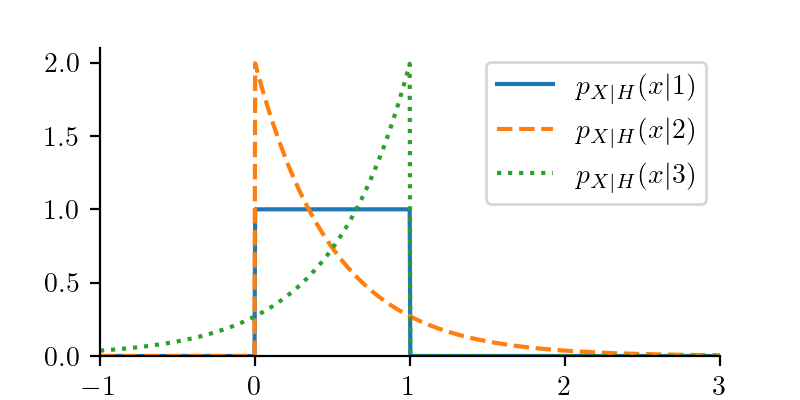
\includegraphics[width=8cm]{Figuras/Px15_3class_likelihoods.png}
\end{center}

El punto de corte de las verosimilitudes de las hipótesis 1 y 2 está dado por la solución de 
\begin{align*}
p_{X|H}&(x|1) = p_{X|H}(x|2)  \\
   &\Leftrightarrow  1 = 2\exp(-2x) \\
   &\Leftrightarrow  x = \frac{\ln(2)}{2} \approx 0.35 
\end{align*}
Del mismo modo (y también por la simetría de  las distribuciones, es inmediato comprobar que el punto de corte de las verosimilitudes de las hipótesis 1 y 3 es
$$
x = 1 - \frac{\ln(2)}{2} \approx 0.66
$$
por tanto, la regla de decisión del decisor bayesiano será
$$
D = \left[
\begin{array}{ll} 
1, & \quad x \in (0.5 \ln(2), \, 1 - 0.5\ln(2))                 \\
2, & \quad x \in [0, \, 0.5\ln(2)] \cup [1, \, \infty)   \\
3, & \quad x \in (-\infty, \, 0] \cup [1-0.5\ln(2),\, 1]
\end{array}
\right.
$$
\part
\begin{align*}
P\{D=1|H=1\} &= P\{x \in (0.5 \ln(2), \, 1 - 0.5\ln(2)) |H=1\} \\
             &= \int_{0.5 \ln(2)}^{1 - 0.5\ln(2)} 1 \cdot dx \\
             &= 1 - \ln(2) \approx 0.31
\end{align*}
Analogamente
\begin{align*}
P\{D=2|H=2\} &= \int_0^{0.5 \ln(2)} 2\exp(-2x) dx + \int_1^{\infty} 2\exp(-2x) dx  \\
             &= \left[ -\exp(-2x) \right]_0^{0.5 \ln(2)} 
              + \left[ -\exp(-2x) \right]_1^{\infty}  \\
             &= \frac12 + e^{-2} \approx 0.64
\end{align*}
y, por simetría
\begin{align*}
P\{D=3|H=3\} = \frac12 + e^{-2} \approx 0.64
\end{align*}

\part Las verosimilitudes de las nuevas hipótesis son:
\begin{align*}
p_{X|H}(x|0) &= (p_{X_2} \ast p_{X_3})(x) = \exp\left(-2|x - 1|\right)   \\
p_{X|H}(x|1) &= p_{X_1}(x)
\end{align*}
(donde $\ast$ denota el operador de convolución), y se representan en la figura
\begin{center}
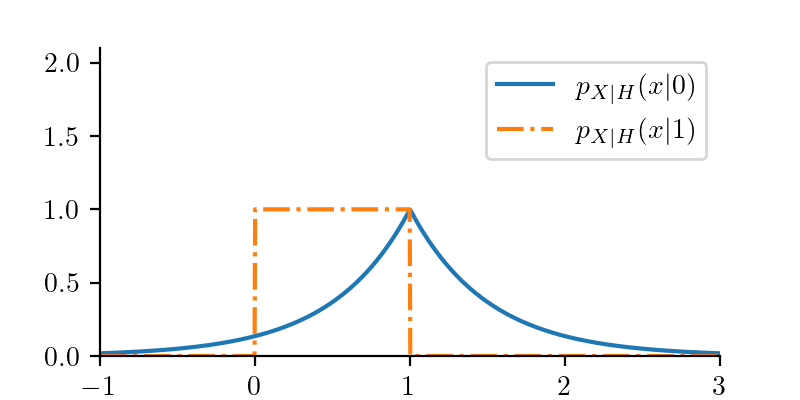
\includegraphics[width=8cm]{Figuras/Px15_2class_likelihoods.png}
\end{center}
Por tanto, el decisor ML será
$$
D = \left[
\begin{array}{ll} 
0, & \quad x \notin    [0, \, 1]    \\
1, & \quad x \in [0, \, 1]
\end{array}
\right.
$$

\part 
\begin{align*}
P_{\rm FA} 
   &= P\{D=1|H=0\} = P\{ 0\le x \le 1 | H=0 \} \\
   &= \int_0^1 \exp(2x-2) dx  
    = \frac12(1 -  e^{-2}) 
    \approx 0.4323
\end{align*}
\begin{align*}
P_{\rm M}=P\{D=0|H=1\} = P\{ x \notin [0, 1] | H=1 \}  = 0
\end{align*}
\end{parts}

\end{solution}
%%%%%%%%%%%%%%

\else

\question Three random variables are characterized by the following likelihoods:
 $$ \begin{array}{l} 
 p_{X_1}(x_1) = \left\lbrace  \begin{array}{ll} 1, & 0 \le x_1 \le 1 \\
 0, & \mbox{otherwise}    \end{array}      \right. \\ \\
 p_{X_2}(x_2) = 2\exp \left( -2x_2  \right), \quad x_2 \ge 0 \\ \\
 p_{X_3}(x_3) = 2\exp \left( 2 \left( x_3-1 \right)   \right), \quad x_3 \le 1 
 \end{array}$$
Considering the following three hypotheses:
 $$ \begin{array}{ll} 
 H=1: & \quad X=X_1\\
 H=2: & \quad X=X_2\\
 H=3: & \quad X=X_3\\
  \end{array}$$
obtain:
\begin{parts}

\part The Bayesian decision-maker that minimizes the overall risk when all hypotheses are {\em a priori} equally probable, and the cost policy is $c_{ii}=0$, $i=1, 2, 3$ and $c_{ij}=c$ with $i\neq j$.
\part Probabilities of deciding $D=i$ given hypothesis $H=i$, i.e., $P\{D=i|H=i\}$ for $i=1, 2, 3$.
\end{parts}
Considering now the binary decision problem characterized by:
  $$ \begin{array}{ll} 
 H=1: & \quad X=X_1\\
 H=0: & \quad X=X_2+X_3
  \end{array}$$
obtain:
\begin{parts}
\setcounter{partno}{2}
\part The corresponding ML classifier.
\part The false alarm and missing probabilities, $P\{D=1|H=0\}$ and $P\{D=0|H=1\}$, respectively.
\end{parts}


%%%%%%%%%%%%%%%%
\begin{solution}
\begin{parts}
\part
Since the costs for all types of error are equal and the cost of hitting is 0, the Bayesian decision-maker is MAP. Also, since the hypothesis are equally likely, the MAP decision-maker is also ML.

According to the statement, the likelihoods of the hypothesis are
\begin{align*}
p_{X|H}(x|1) = p_{X_1}(x) \\
p_{X|H}(x|2) = p_{X_2}(x) \\
p_{X|H}(x|3) = p_{X_3}(x) 
\end{align*}
and they are represented in the figure.
\begin{center}
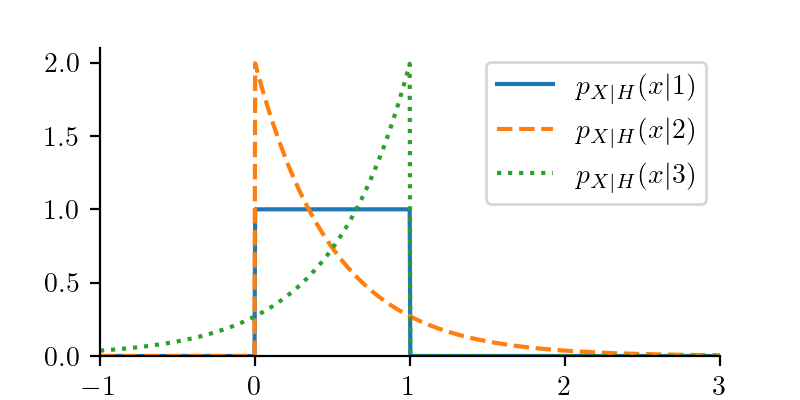
\includegraphics[width=8cm]{Figuras/Px15_3class_likelihoods.png}
\end{center}

The cutting point of the likelihoods for hypotheses 1 and 2 is given by the solution of
\begin{align*}
p_{X|H}&(x|1) = p_{X|H}(x|2)  \\
   &\Leftrightarrow  1 = 2\exp(-2x) \\
   &\Leftrightarrow  x = \frac{\ln(2)}{2} \approx 0.35 
\end{align*}
in the same way (an also because of the symmetry of the distributions) it is straightforward to verify that the cut point of the likelihoods for hypotheses 1 and 3 is
$$
x = 1 - \frac{\ln(2)}{2} \approx 0.66.
$$
Thus, the Bayesian decision rule is
$$
D = \left[
\begin{array}{ll} 
1, & \quad x \in (0.5 \ln(2), \, 1 - 0.5\ln(2))                 \\
2, & \quad x \in [0, \, 0.5\ln(2)] \cup [1, \, \infty)   \\
3, & \quad x \in (-\infty, \, 0] \cup [1-0.5\ln(2),\, 1]
\end{array}
\right.
$$
\part
\begin{align*}
P\{D=1|H=1\} &= P\{x \in (0.5 \ln(2), \, 1 - 0.5\ln(2)) |H=1\} \\
             &= \int_{0.5 \ln(2)}^{1 - 0.5\ln(2)} 1 \cdot dx \\
             &= 1 - \ln(2) \approx 0.31
\end{align*}
Analogamente
\begin{align*}
P\{D=2|H=2\} &= \int_0^{0.5 \ln(2)} 2\exp(-2x) dx + \int_1^{\infty} 2\exp(-2x) dx  \\
             &= \left[ -\exp(-2x) \right]_0^{0.5 \ln(2)} 
              + \left[ -\exp(-2x) \right]_1^{\infty}  \\
             &= \frac12 + e^{-2} \approx 0.64
\end{align*}
y, por simetría
\begin{align*}
P\{D=3|H=3\} = \frac12 + e^{-2} \approx 0.64
\end{align*}

\part The likelihoods for the new hypotheses are:
\begin{align*}
p_{X|H}(x|0) &= (p_{X_2} \ast p_{X_3})(x) = \exp\left(-2|x - 1|\right)   \\
p_{X|H}(x|1) &= p_{X_1}(x)
\end{align*}
(where $\ast$ denotes the convolution operator), and they are represented in the figure
\begin{center}
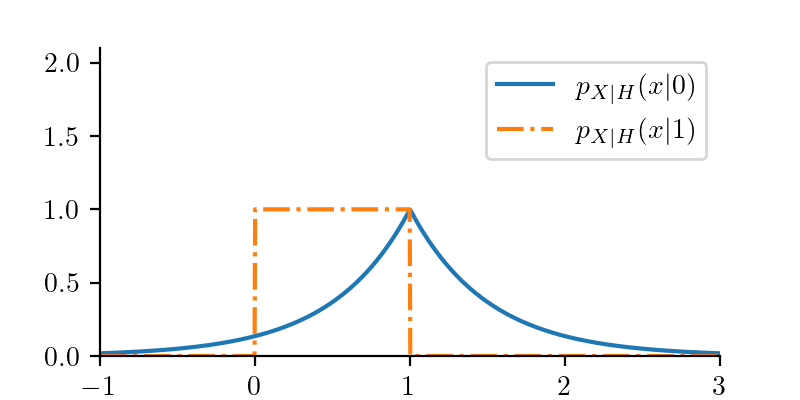
\includegraphics[width=8cm]{Figuras/Px15_2class_likelihoods.png}
\end{center}
Thus, the ML decision-maker is
$$
D = \left[
\begin{array}{ll} 
0, & \quad x \notin    [0, \, 1]    \\
1, & \quad x \in [0, \, 1]
\end{array}
\right.
$$

\part 
\begin{align*}
P_{\rm FA} 
   &= P\{D=1|H=0\} = P\{ 0\le x \le 1 | H=0 \} \\
   &= \int_0^1 \exp(2x-2) dx  
    = \frac12(1 -  e^{-2}) 
    \approx 0.4323
\end{align*}
\begin{align*}
P_{\rm M}=P\{D=0|H=1\} = P\{ x \notin [0, 1] | H=1 \}  = 0
\end{align*}
\end{parts}

\end{solution}
%%%%%%%%%%%%%%

\fi